\chapter{Physical view}

\section{Phase 1: making STIFF real time}

Since the current asynchronousness and overall slowness of the STIFF system
clearly appears to be an obstacle to maximizing business at SureThing, we
recommend taking care of this part of the architecture first. This will
improve the company's yield at an early stage, and therefore will probably
help financing the rest of the operation, as opposed to taking care of the
STIFF system in the last.

\begin{figure}
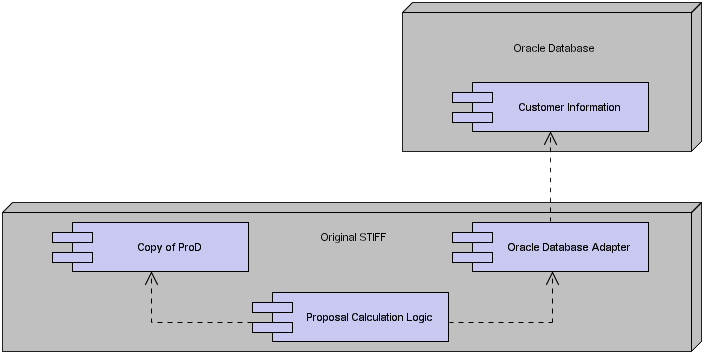
\includegraphics[width=\linewidth]{img/net_1_before.png}
\caption{Current (standalone) STIFF, running overnight}
\label{fig:net_1_before}
\end{figure}

The best way of significantly improving the system's performance as soon as
possible is to provide some kind of quick fix at first, so that proposal
calculation requests are processed \textit{on demand}, until the complete
redesign of the STIFF system is ready for deployment.

\begin{figure}
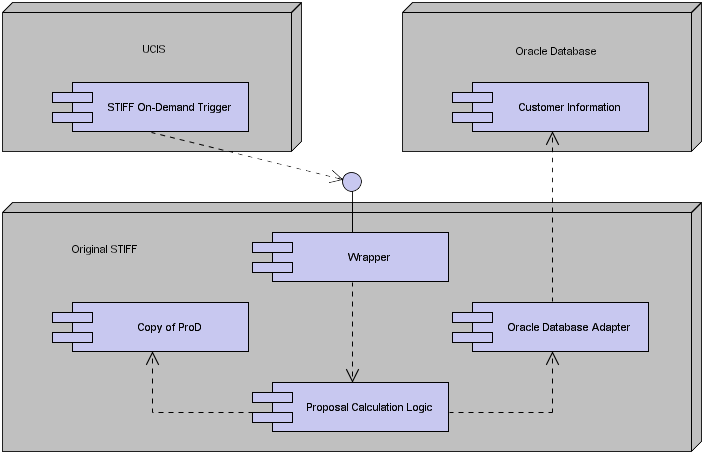
\includegraphics[width=\linewidth]{img/net_1_after.png}
\caption{On-demand STIFF, triggered by UCIS via a temporary wrapper}
\label{fig:net_1_after}
\end{figure}

Another advantage is that by making this in two steps it is possible to
make a minimalistic investment in hardware at first, on which to have the
transitional STIFF system running, and then evaluate the need for extra
computing power required by the real time STIFF system.

\subsubsection*{Cost: about \euro3000}

The most appropriate for a STIFF cluster would be to buy rack servers, so
that space is not wasted by arraying several bulky tower servers.

However, an initial investment of about \euro1000 will be
necessary to buy a rack mount cabinet of capacity between 24 (which is
usually the minimum) and 48 space units (U's). Server racks are then
designated as 1U, 2U and 4U depending on their size.

A study of all the rack server solutions proposed by DELL
has been done, and it would seem that the PowerEdge SC1425 corresponds
the best to this project's needs: it is the most affordable DELL
performance server and it fits in only one rack space unit (1U). It comes
with either one or two processors, but since the old STIFF software was not
designed to run multithreaded it will drain all the power from the first
processor and none of the second one. Therefore we recommend buying a first
PowerEdge SC1425 containing only one processor but the strongest one available
(Intel Xeon EM64T 3.6GHz, 1MB Cache, 800MHz FSB), for a price of
approximately \euro2000.

Note that once the new STIFF software is ready, it will be able to fully
take profit of a multiprocessor system; thus other solutions such as the dual
processor version of the PowerEdge SC1425 rack server based on two similar
but slower (Intel Xeon EM64T 2.8GHz, 1MB Cache, 800MHz FSB) processors will
be more efficient, and at the same time cheaper: around \euro1700 for this
particular solution.

\section{Phase 2: building the web front-end}

Currently, the Call-Center employees use a custom-made UCIS client
for Windows that contains a significant amount of business logic.
This is difficult to maintain because each time that portion of
business logic has to be updated, it has to be updated on every single
computer where the UCIS client is installed.


\begin{figure}
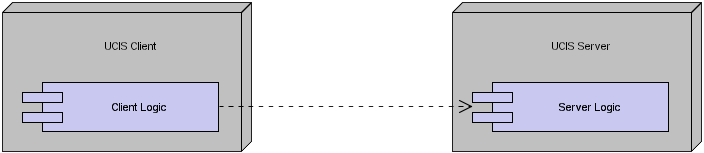
\includegraphics[width=\linewidth]{img/net_2_before.png}
\caption{The UCIS system, with business logic on the client side}
\label{fig:net_2_before}
\end{figure}

Consequently, we recommend centralizing that logic in a website, which
in turn will also free SureThing of all the concerns towards compatibility of
the UCIS client with the various operating system, or various operating system
versions the UCIS users may be running. It helps SureThing into achieving the
Extended Enterprise model by providing a web infrastructure to the
company, a requirement for maximizing cooperation with partners.

\begin{figure}
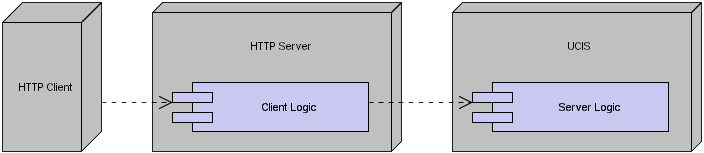
\includegraphics[width=\linewidth]{img/net_2_after.png}
\caption{The UCIS system, with centralized business logic}
\label{fig:net_2_after}
\end{figure}

In order to switch from the UCIS client application for Windows to a
web-based user interface, an investment in dedicated web servers is
required.

\subsubsection*{Cost: about \euro1500}

The main concern on the web servers will be reliability, and not so
performance. Therefore we recommend buying entry-level rack servers
such as the DELL PowerEdge 750, which comes for about \euro1100
when based on a single processor (Intel Celeron processor, 2.4GHz,
128K Cache, 400MHz FSB) and 1GB of memory.

A single PowerEdge 750 will be sufficient to handle the initial load
generated by the traffic of ex-users of the UCIS client for Windows
on the website. And once the company's commitment in the e-commerce
world broadens, attracting more and more visitors to the website, it
will be easy to add one or several other PowerEdge 750 units to the
rack mount cabinet shared with the STIFF server array.

\section{Phase 3: finalizing a minimalistic but scalable architecture}

At this point it will already be possible to have an early estimation
about the computing power required by the transitional on-demand STIFF
system, and eventually invest in one or several other PowerEdge SC1425
units to cope with the future load of the final STIFF system.
As said earlier, the final STIFF system will be capable of multithreading
and it would then be profitable to buy performance rack servers based on
2 to 4 processors, to get the fastest response time per machine of the
cluster.

\begin{figure}
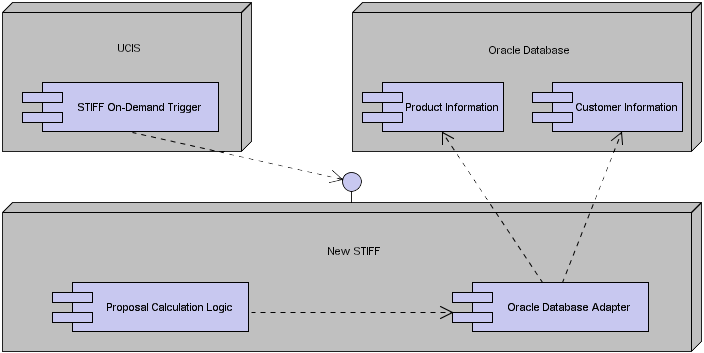
\includegraphics[width=\linewidth]{img/net_3.png}
\caption{The final STIFF system}
\label{fig:net_3}
\end{figure}

Also, since it is likely that the STIFF system will need a fast connection
to the Oracle database once the product information is moved from ProD
to the former, and since the network traffic will significantly increase
with the company's growth, we recommend upgrading the network infrastructure
to support communications at a speed of at least one gigabit per second (1Gbps).

\subsubsection{Cost: about \euro5000}

The new rack servers already come with gigabit network adapters, so the cost
will mostly be implied by upgrading existing hardware and cabling, and also
centralizing the servers in the same location to benefit from Local Area
Network (LAN) connectivity.

\section{Phase 4: achieving zero-downtime}

The idealistic network architecture for SureThing, in order to satisfy
performance and reliability needs, would be something like this:\\

\begin{figure}
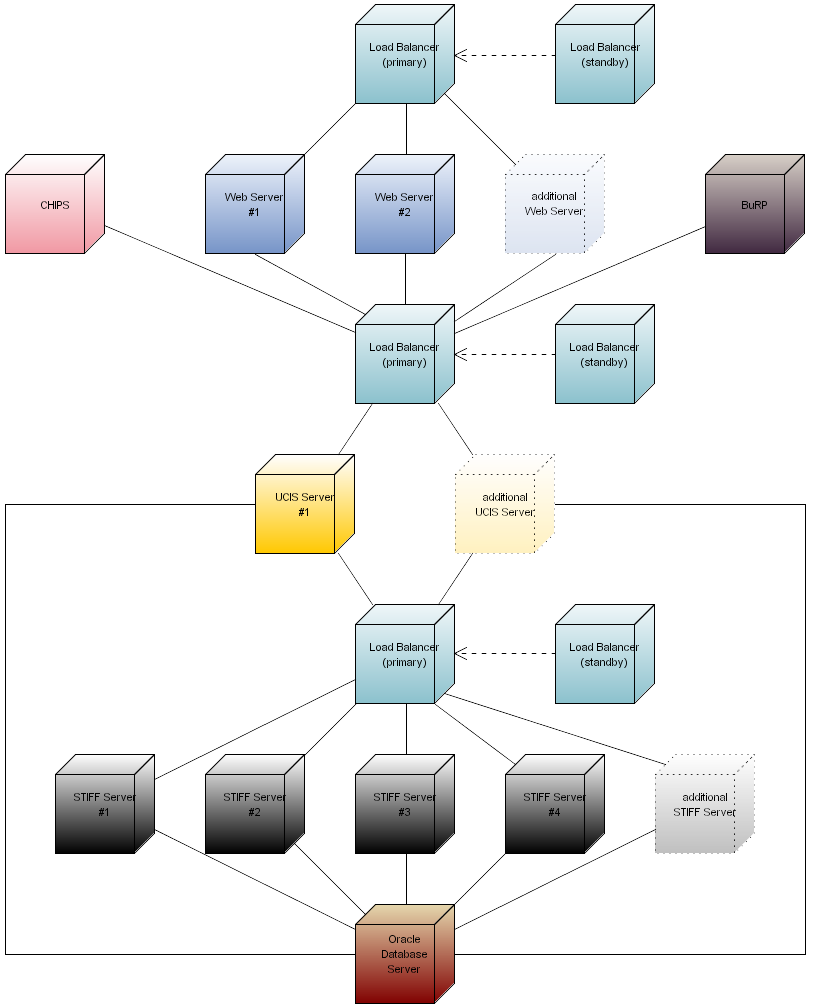
\includegraphics[width=\linewidth]{img/net_4.png}
\caption{Ideal network configuration}
\label{fig:net_4}
\end{figure}

Note that only one box was drawn for the CHIPS system, when actually there
can be several CHIPS applications interacting with the UCIS system, but we
believe that it is not relevant in this view. Same with the BuRP system.\\

The load balancers will make it possible to spread the load across a cluster
of several computers performing the same task, designated as "nodes" of the
cluster. Concretely, thel load balancers will be hardware such as the Coyote Point Equalizer
E250i, available for approximately \euro3000 a piece. There are cheaper
load-balancing solutions, but this particular one is capable of distributing
the load unevenly between computers of different capabilities, and as an
extension of this, is also capable of detecting node failures and immediately
stop forwarding connections to affected nodes.

The "standby" load balancer attached to each of the "primary" load balancers
is there to provide redundancy in case of failure of the primary, completing
the system's insurance of zero-downtime.

The Oracle database is different: for all the other systems the risk is mainly
of the system's logic to fail and loss of data on those has no significant
consequence, whereas for the database, the data is crucial because it represents
company information that has been accumulated in years of business... The risk
of software failure on the Oracle server has to be considered minimal, according
to its vendor's slogan: "Oracle, the unbreakable database", and anyway it would
be quite difficult to provide redundancy for the system at the software level.
However, hardware redundancy can easily be achieved by duplicating each hard disk
drive using RAID technology, which would provide zero-downtime recovery in case
of hard disk drive failure. Furthermore, also making back-ups of the database on
tapes and storing those at another location would prevent loss of data in case
of major disasters such as fire in server room.

\subsubsection{Cost: about \euro30000}

\begin{description}
\item[\euro9000] primary load balancers
\item[\euro1000] second web server for system redundancy
\item[\euro1500] second UCIS server for system redundancy
\item[\euro2000] second STIFF server for system redundancy
\item[\euro3500] RAID array on Oracle server for hardware redundancy
\item[\euro3000] tape drive + sufficient set of blank tapes for backups
\item[\euro9000] extra load balancers for network redundancy
\end{description}

Note that \textbf{these are all optional and can be invested in at any time};
the capital budgeting decision in regard to the insurance of zero-downtime is
up to SureThing's managers.